\documentclass[12pt,a4paper,twoside,openright]{report}
\usepackage[pdfborder={0 0 0}]{hyperref}    % turns references into hyperlinks
\usepackage[margin=25mm]{geometry}  % adjusts page layout
\usepackage{graphicx}  % allows inclusion of PDF, PNG and JPG images
\usepackage{verbatim}
\usepackage{docmute} 
\usepackage[utf8]{inputenc}
\usepackage[english]{babel}
\usepackage{graphicx}
\usepackage{wrapfig}
\usepackage{float}
\usepackage{booktabs}
\usepackage{tabularx}
\usepackage{multirow}
\usepackage{longtable}
\usepackage{amsmath}
\usepackage{makecell}
\usepackage{amssymb}
\usepackage{calrsfs}
\usepackage{diffcoeff}
\usepackage{mathtools}
\usepackage{amsfonts}
\usepackage{float}
\usepackage[T1]{fontenc}
\usepackage{currvita}
\usepackage[none]{hyphenat}
\usepackage{algorithm}
\usepackage[noend]{algpseudocode}
\usepackage{listings}
\usepackage{xcolor}
\usepackage{natbib}
\usepackage{subcaption}
\usepackage{colortbl}
\usepackage{hhline}
\usepackage{enumitem}

\DeclareMathOperator*{\argmax}{arg\,max}
\DeclareMathOperator*{\argmin}{arg\,min}


\makeatletter
\def\@documentnocite#1{\@bsphack
  \@for\@citeb:=#1\do{%
    \edef\@citeb{\expandafter\@firstofone\@citeb}%
    \if@filesw\immediate\write\@auxout{\string\citation{\@citeb}}\fi
    \@ifundefined{b@\@citeb}{\G@refundefinedtrue
      \@latex@warning{Citation `\@citeb' undefined}}{}}%
  \@esphack}
\AtBeginDocument{\let\nocite\@documentnocite}

\algdef{SE}[DOWHILE]{Do}{doWhile}{\algorithmicdo}[1]{\algorithmicwhile\ #1}%


\makeatother


\DeclareMathOperator*{\argmax}{arg\,max}
\DeclareMathOperator*{\argmin}{arg\,min}

\setcounter{secnumdepth}{5}
\raggedbottom                           % try to avoid widows and orphans
\sloppy
\clubpenalty1000%
\widowpenalty1000%

\renewcommand{\baselinestretch}{1.1}    % adjust line spacing to make
                                        % more readable
      
      
 \colorlet{punct}{red!60!black}
 \definecolor{background}{HTML}{EEEEEE}
 \definecolor{delim}{RGB}{20,105,176}
 \colorlet{numb}{magenta!60!black}
                                   
 \lstdefinelanguage{json}{
  basicstyle=\normalfont\ttfamily,
  numbers=left,
  numberstyle=\scriptsize,
  stepnumber=1,
  numbersep=8pt,
  showstringspaces=false,
  breaklines=true,
  frame=lines,
  backgroundcolor=\color{white},
  literate=
  *{0}{{{\color{numb}0}}}{1}
  {1}{{{\color{numb}1}}}{1}
  {2}{{{\color{numb}2}}}{1}
  {3}{{{\color{numb}3}}}{1}
  {4}{{{\color{numb}4}}}{1}
  {5}{{{\color{numb}5}}}{1}
  {6}{{{\color{numb}6}}}{1}
  {7}{{{\color{numb}7}}}{1}
  {8}{{{\color{numb}8}}}{1}
  {9}{{{\color{numb}9}}}{1}
  {:}{{{\color{punct}{:}}}}{1}
  {,}{{{\color{punct}{,}}}}{1}
  {\{}{{{\color{delim}{\{}}}}{1}
  {\}}{{{\color{delim}{\}}}}}{1}
  {[}{{{\color{delim}{[}}}}{1}
  {]}{{{\color{delim}{]}}}}{1},
 }

\newcommand{\HRulee}{\rule{\linewidth}{0.5mm}}

 
\begin{document}

\bibliographystyle{plain}


%%%%%%%%%%%%%%%%%%%%%%%%%%%%%%%%%%%%
%%%%%%%%%%%%%%% TITLE %%%%%%%%%%%%%%%%%
%%%%%%%%%%%%%%%%%%%%%%%%%%%%%%%%%%%%

\pagestyle{empty}

\rightline{\LARGE \textbf{Tiberiu-George Copaciu}}

\vspace*{60mm}
\HRulee
\begin{center}

  \Huge
  \textbf{Descriptive file names from content and context} \\[5mm]
  Computer Science Tripos -- Part II \\[5mm]
  Homerton College \\[5mm]
  \today  % today's date
\end{center}
\HRulee
\begin{figure}[H]
  \centering
  
\includegraphics[scale = 0.5]{Images/logo2.jpg}
\end{figure}

%%%%%%%%%%%%%%%%%%%%%%%%%%%%%%%%%%%%
%%%%%%%%%%%% PROFORMA %%%%%%%%%%%%%%%%
%%%%%%%%%%%%%%%%%%%%%%%%%%%%%%%%%%%%

\pagestyle{plain}

\chapter*{Proforma}

{\large
  \begin{tabular}{ll}
    Name:               & \bf Tiberiu-George Copaciu                          \\
    College:            & \bf Homerton College                                \\
    Project Title:      & \bf Descriptive file names from context and content \\
    Examination:        & \bf Computer Science Tripos -- Part II, July 2019   \\
    Word Count:         & \bf $\mathbf{0}$\footnotemark[1]                    \\
    Project Originator: & Dr Lucian Carata                                    \\
    Supervisor:         & Dr Lucian Carata                                    \\
  \end{tabular}
}

\footnotetext[1]{This word count was computed
  using TexCount: \url{https://app.uio.no/ifi/texcount/}}

\section*{Original aims of the project}

This project aims to give a solution to the problem of files created either by users or processes which end up having unintuitive/non-descriptive names. Thus, the core goal of the project was to implement a machine learning pipeline capable of classifying files in terms of their content and context (graphs representing provenance data) information. Afterwards, using this results and a user-given policy, the project should rename/reorganise files and present them to the user into a virtual filesystem. 

\section*{Work completed}

\section*{Special Difficulties}
None.

\newpage
\section*{Declaration}
I, Tiberiu-George Copaciu of Homerton College,
being a candidate for Part II of the Computer Science Tripos,
hereby declare that this dissertation and the work described in it
are my own work, unaided except as may be specified below, and
that the dissertation does not contain material that has already
been used to any substantial extent for a comparable purpose.
\\ \\
Signed

\includegraphics[height=1.5\baselineskip]{Images/signature.jpg}
\\ \\
Date \today

\newpage
\tableofcontents
\listoffigures
\listoftables
\newpage
\section*{Acknowledgements}

I would like to express my deepest appreciation to my supervisor, Dr Lucian Carata, for his patient and persistent guidance, encouragement and advice provided throughout my time working for this project. I would also like to thank my Director of Studies, Dr John Fawcett, for his help and support during my entire undergraduate degree. Finally, this project and student journey would have not been possible without the emotional support of my family and my girlfriend, who have always encouraged me in all my pursuits. 

\begin{document}

\chapter{Introduction}

This project aims to make use of, re-implement and adapt machine learning techniques in order to identify, classify, and rename files from distributed systems, which end up having un-intuitive names. These names can be the result of either intentional activity (e.g. be created by attackers to disguise the actual contents of files before exfiltration, concatenate data from multiple files before exfiltration) or appear organically as part of the using system (e.g. running of scripts and experiments that use temporary file names which are not deleted, files produced by the simulated developers when downloading documentation or new software from the internet). \\


\section{Aims and Motivation}  \label{1.1}

In order to develop a set of features for the intended classification pipeline, the project will use a couple of different sources of information about the target files. Firstly, a typical approach involving file classification with respect to their content is implemented. Secondly, to generate further features, and as an element of novelty, I will use system traces which highlight the relation between programs and data objects, stored in the format of a graph database. In these \textit{provenance graphs}, nodes represent entities such as files, processes, sockets, pipes, while edges are recording, at a fine grained level, influences between the nodes. Thus, at the core of the project there is a graph classification pipeline. Specifically, the Patchy-San$^{\small \cite{Patchy-San}}$ algorithm is used in combination with a convolutional neural network to achieve the desired result. As a final stage of the project, I have implemented files re-naming based on user-given policy and by using the acquired classification information, presenting the user the renaming proposals (as opposed to intervening on the files directly). \\

The provided provenance dataset is a result of the \textit{Observational Provenance in User Space} (OPUS) research project$^{\small \cite{OPUS}}$, and these system traces are taken from machines on which typical developer/attacker behaviour is simulated. Thus, while everything is made to look similar to normal user behaviour, these are not genuine activities or sensitive data being exfiltrated. Hence, neither privacy nor ethics are a primary concern. \\

The point of the project is to explore how/with what degree of success can machine learning be deployed to deal with the naming/structuring issues mentioned above. Not applying machine learning means one has to know a lot more about what executes on the system and the types of files or the types of activity that generates them. The exercise here is to see how well a ML algorithm can start reducing the amount of knowledge needed from analysts when looking at an arbitrary system. In short, it is a trade-off: one can apply non-ML approaches on this particular dataset if you start by knowing the ground truth or the types of activities that run on the system, but it's unclear whether a ML approach could do just as well while requiring less anterior knowledge. The goal is to design a ML pipeline to test this hypothesis out and give an answer to the question. \\

\section{Challenges}

One obstacle was the lack of enough provenance training data and examples of suggestible patterns that could be fed as input to the ML models. To overcome this, synthetic data was created by generating variations of graphs which mimic the original dataset. This process is described in detail in Section \ref{Synthetic Data Generation}.

\section{Related Work}

This section discusses various approaches on individual sub-tasks of the project. Each of the ideas presented is contrasted with the project's requirements, explaining whether it is a viable option for its purposes or not. \\

\subsection{Document Classification}

Document Classification is an important and typical tasks in supervised machine learning. Assigning categories to documents, which can be a web page, library book, media articles, gallery etc. has many applications, e.g. spam filtering, email routing, sentiment analysis. The bag-of-words$^{\small \cite{BOW}}$ model is commonly used in methods of document classification where the (frequency of) occurrence of each word is used as a feature for training a classifier such as Naive Bayes$^{\small \cite{NaiveBayes}}$ or Support Vector Machines$^{\small \cite{SVM}}$. This model is a simplifying representation used in natural language processing in which a text (such as a sentence or a document) is converted into a bag (multiset) of its own words, disregarding grammar and even word order, but keeping multiplicity. \\

This approach has been successfully used for human written documents. However, my project rather aims to classify file generated by various programs and processing pipelines, which will probably require different or improved techniques. \\

\subsection{File Renaming using Metadata}

There exists a large variety of tools designed to automatise the file renaming task. One such tool called \textit{Rename Expert} implements a considerable amount of features of interest. For instance:

\begin{itemize}
  \item metadata (EXIF, IPTC, ID3, etc.) can be used for the naming of files (e.g., for images, video files or audio files).
  \item automatically rename text files based on a part of the file contents (e.g., to include data from TXT, XML, HTML, or log files).
  \item simultaneously rename folders along with subfolders and files - allows the batch renaming of any number of files and folders in one go.
\end{itemize}

The downside of this category of programs is that they require extensive user involvement and detailed knowledge of the target system. In contrast, the project desires to reduce as much as possible the effort and contribution of a specialist by using appropriate machine learning techniques. Moreover, this project is inclined towards more generality, being less dependent of files' metadata. \\


\subsection{Graph Kernels}

Graph Kernels$^{\small \cite{GraphKernels}}$ make kernel machines such as SVMs feasible for graph classification by computing some positive semidefinite graph similarity measures, which have achieved state-of-the-art classification results on many graph datasets. Most existing graph kernels focus on comparing small local patterns. Deep graph kernels learn latent representations of substructures (walks, paths, subtrees) to leverage their dependency information. Convolution kernels compare two graphs based on all pairs of their substructures. Assignment kernels, on the other hand, tend to find a correspondence between parts of two graphs. \\

In contrast to these computationally expensive approaches, the proposed Patchy-San algorithm is time efficient and highly parallelisable, as will be discussed in Section \ref{Evaluation Results}.

\end{document}
\begin{document}

\chapter{Preparation}

The Preparation chapter presents the fundamental theory which serves as bases on which the algorithms in this project are developed. It explores the requirement analysis and software engineering strategies such that the project successfully achieves and (possibly) surpasses the success criteria. All the work described in this chapter is prior to any actual implementation.


\section{Introduction to Neural Networks}

An Artificial Neural Network (ANN) is a computational model that is inspired by the way biological neural networks in the human brain process information. Artificial Neural Networks have generated a lot of excitement in Machine Learning research and industry, thanks to many breakthrough results in speech recognition, computer vision and text processing.

\subsection{Artificial Neuron}

The basic unit of computation in a NN is the Artificial Neuron. A neuron receives input either directly from the dataset or from another neuron and combines it with a set of coefficients, known as weights, thereby assigning significance to inputs with regard to the task the algorithm is trying to learn. These input-weight products are summed and then passed through an activation function $\sigma : \mathbb{R} \rightarrow \mathbb{R}$ as can be observed in Figure \ref{Artificial Neuron}. The additional bias that is generated by each neuron allows shifting the activation function to the left or to the right. \\

\begin{figure}[H]
  \centering
  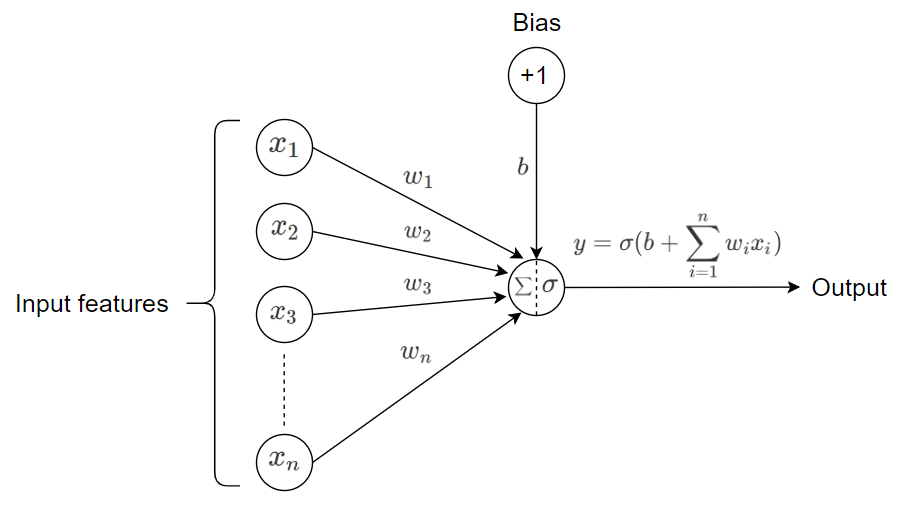
\includegraphics[scale = 0.5]{Images/artificial_neuron.png}
  \caption{Artificial Neuron Structure.}
  \label{Artificial Neuron}
\end{figure}

The purpose of an activation function is to introduce non-linearity into a NN, in the sense that the output will not be always represented as a linear combination of the inputs. Hence, it increased the expresivity and the diversity of functions that can be learnt by a NN. Some popular activation functions are listed below:\\

\begin{itemize}
  \item the sigmoid/logistic function: \\
        \begin{equation}
          \sigma(x) = \frac{1}{1 + e^{-x}}
        \end{equation}

  \item the hyperbolic tanget function: \\
        \begin{equation}
          \sigma(x) = tanh(x) = \frac{e^{x} - e^{-x}}{e^{x} + e^{-x}}
        \end{equation}

  \item the Rectified Linear Unit (ReLU) function: \\
        \begin{equation}
          \sigma(x) = max(0,x)
        \end{equation}
\end{itemize}


\subsection{Multilayer Perceptron}

A Multilayer Perceptron (MLP) is a finite, directed, acyclic graph in which the nodes represent artificial neurons and they are arranged in at least three layers. Nodes that are no target of any connection are called input neurons and represent input features. Nodes that are no source of any connection are called output neurons and represent predictions for the possible classes. Nodes that are neither input nor output neurons are called hidden neurons. The organisation of nodes in layers implies that nodes belonging to layer $i$ in the MLP serve as input features for nodes in layer $i+1$. \\

The most distinctive feature of MLPs is that they are fully connected NNs: each node in layer $i$ is connected to each node in layer $i+1$.

\begin{figure}[H]
  \centering
  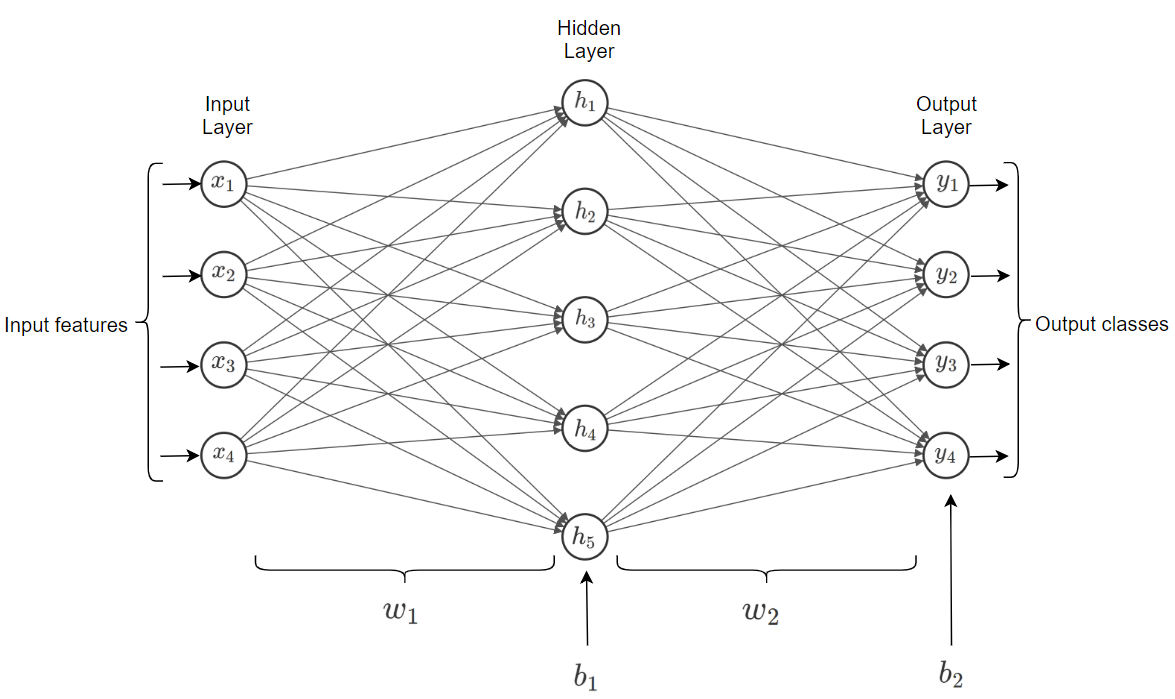
\includegraphics[scale = 0.5]{Images/mlp.png}
  \caption{Multilayer Perceptron Structure.}
  \label{Multilayer Perceptron}
\end{figure}

\subsection{Convolutional Neural Networks}

For some types of data, especially for images, MLPs are not the most appropriate approach. Indeed, they are defined on vectors as input data, which means, we shall transform images into vectors in order to apply MLPs, loosing the way spatial information is contained. \\\

In contrast to the baseline model of MLP, a Convolutional Neural Network (CNN) uses a specialised architecture (applied directly on matrices), well-adapted for image classification. A CNN is able to successfully capture the spatial dependencies in an image through the application of relevant filters. The architecture performs an adequate fitting to an image dataset due to the reduction in the number of parameters involved and re-usability of weights. A typical CNN is comprised of convolutional, pooling and dense layers. \\

\subsubsection*{Convolutional Layers}

Convolution is a specialised type of linear operation used for feature extraction, where a small array of numbers, called a kernel, is applied across the input, which is an array of numbers, called a tensor. An element-wise product between each element of the kernel and the input tensor is calculated at each location of the tensor and summed to obtain the output value in the corresponding position of the output tensor, called a feature map. This is illustrated in Figure \ref{Convolution}. This procedure is repeated applying multiple kernels to form an arbitrary number of feature maps, which represent different characteristics of the input tensors; different kernels can, thus, be considered as different feature extractors. The first convolution layer extracts low-level features like edges, lines, and corners. Higher-level layers extract higher-level features. \\

\begin{figure}[H]
  \centering
  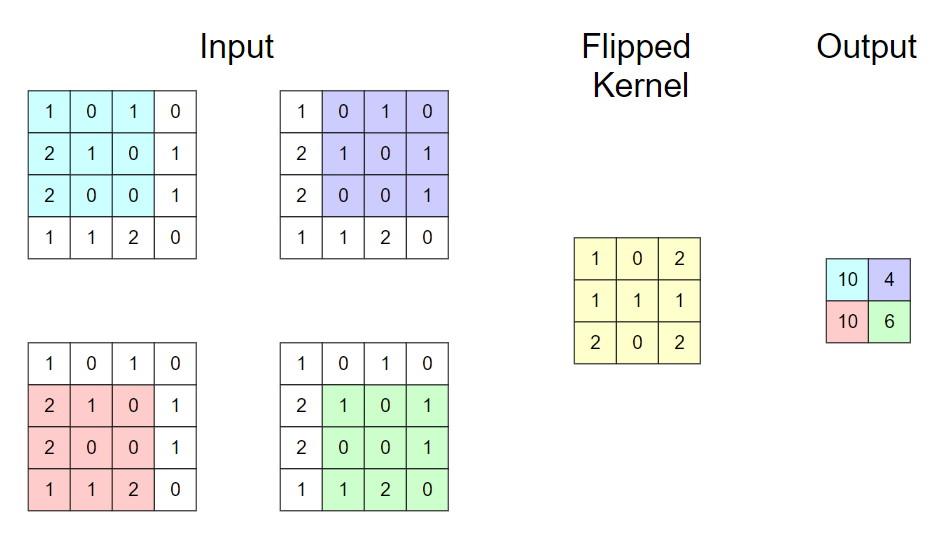
\includegraphics[scale = 0.6]{Images/convolution.png}
  \caption{Example of a Convolution operation where coloured areas of the input matrix are successively dot producted with the flipped kernel.}
  \label{Convolution}
\end{figure}

Formally, given the image size N*M and the kernel size L1*L2, the 2D discrete convolution is described by the following equation: \\

\begin{equation}
  \text{Convolution}_{ij} = \sum_{l_1=0}^{L1-1} \sum_{l_2=0}^{L2-1} K[l_1][l_2]*I[i+l_1][j+l_2]
\end{equation}
$$\text{where} \ 0 \leq i < N \ \text{and} \ 0 \leq j < M$$ \\

The convolution operation described above does not allow the center of each kernel to overlap the outermost element of the input tensor, and reduces the height and width of the output feature map compared to the input tensor. Padding, typically zero padding, is a technique to address this issue, where rows and columns of zeros are added on each side of the input tensor, so as to fit the center of a kernel on the outermost element and keep the same in-plane dimension through the convolution operation. \\

The key feature of a convolution operation is weight sharing: kernels are shared across all the image positions. Weight sharing creates the following characteristics of convolution operations: (1) letting the local feature patterns extracted by kernels translation b invariant as kernels travel across all the image positions and detect learned local patterns, (2) learning spatial hierarchies of feature patterns by subsampling in conjunction with a pooling operation, resulting in capturing an increasingly larger field of view, and (3) increasing model efficiency by reducing the number of parameters to learn in comparison with fully connected neural networks. \\


\subsubsection*{Pooling Layers}

Pooling is a procedure that reduces the input over a certain area to a single value (subsampling). An illustration of pooling can be found in Figure \ref{Pooling}. In convolutional neural networks, this concentration of information provides similar information to outgoing connections with reduced memory consumption. Pooling provides basic invariance to rotations and translations and improves the object detection capability of convolutional networks. For example, the face on an image patch that is not in the center of the image but slightly translated, can still be detected by the convolutional filters because the information is funneled into the right place by the pooling operation. The larger the size of the pooling area, the more information is condensed, which leads to slim networks that fit more easily into memory. However, if the pooling area is too large, too much information is thrown away and predictive performance decreases. \\

\begin{figure}[H]
  \centering
  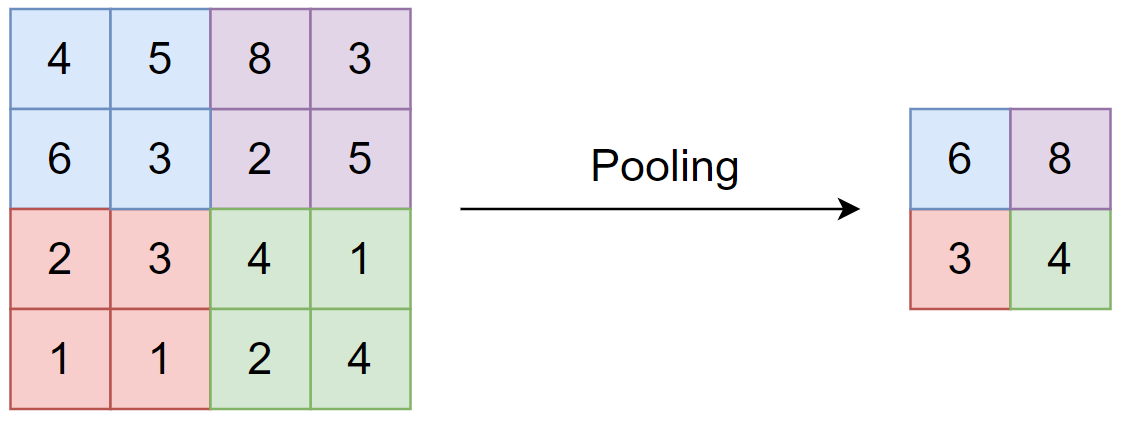
\includegraphics[scale=0.3]{Images/pooling.png}
  \caption{Example of Max Pooling operation with 2 by 2 kernel size and stride 2.}
  \label{Pooling}
\end{figure}

\subsubsection*{Fully Connected Layers}

After several convolution and pooling layers, the CNN usually ends with multiple fully connected layers. The output from the convolutional and pooling layers represent high-level features of the input image. The purpose of the dense layers is to use these flattened features for classifying the input image into various classes based on the training dataset. \\

\subsection{Supervised Learning using Neural Networks}

As the main goal of the project is a classification task, in this section I will present how NNs can be used to achieve this and the mathematical background behind training and predicting stages. \\\

To begin with, supervised learning requires a given training set S = \{ ($x_1$,$y_1$), ($x_2$,$y_2$), ... , ($x_n$,$y_n$) \}, where \textbf{$x_i$} is a feature vector of the entity we are interested to classify and \textbf{$y_i$} is a one hot encoding of the class to which \textbf{$x_i$} corresponds. Given S, a NN with some established architecture and some weights \textbf{w} and biases \textbf{b}, essentially represents a function f(\textbf{x},\textbf{w},\textbf{b}) which outputs an estimated class for an input feature vector \textbf{x}. Thus, we can define h : $\mathbb{R}^m \rightarrow \textit{C}$ (where \textit{C} is the set of all possible output classes) h(\textbf{x}) = f(\textbf{x}, \textbf{w}, \textbf{b}) that provides us with the required classification.

\subsubsection*{Training}

Before explaining the training procedure, the notion of a loss function must be defined. That is, a function computing the magnitude of the error between the NN's class prediction and the real class. One of the most popular loss functions for classification purposes is cross-entropy.

\begin{equation}
  \mathbf{\mathfrak{L}}(\mathbf{w}, \mathbf{b}, \mathbf{x_i}, \mathbf{y_i}) = - \sum_{j=1}^k y_{i,j} \ ln(y'_{i,j})
\end{equation}

The training stage starts by randomly initialising the weights and biases of the NN and computing an initial value of the loss function. Afterwards, the gradient descent optimisation algorithm$^{\small \cite{gradient_descent}}$ is used to minimise the value of the loss function (i.e. improve the prediction capabilities of the network). Using this algorithm, iteratively, more appropriate values for weights and biases are determined. \\

\begin{equation}
  \mathbf{w_{t+1}} \leftarrow \mathbf{w_t} - \alpha \sum_{i=1}^m \frac{\partial \mathfrak{L}}{\partial \mathbf{w}}\Bigr|_{\substack{\mathbf{w}_t}}
\end{equation}

\begin{equation}
  \mathbf{b_{t+1}} \leftarrow \mathbf{b_t} - \alpha \sum_{i=1}^m \frac{\partial \mathfrak{L}}{\partial \mathbf{b}}\Bigr|_{\substack{\mathbf{b}_t}}
\end{equation}

\bigskip

An important parameter in Gradient Descent is the size of the steps, determined by the learning rate hyperparameter. If the learning rate is too small, then the algorithm will have to go through many iterations to converge, which will take a long time (LHS of Figure \ref{learnrate}). On the other hand, it the learning rate is too high, this might cause the algorithm to diverge, never reaching the intended minimum, loss function values becoming greater and greater (RHS of Figure \ref{learnrate}). \\

\begin{figure}[H]
  \centering
  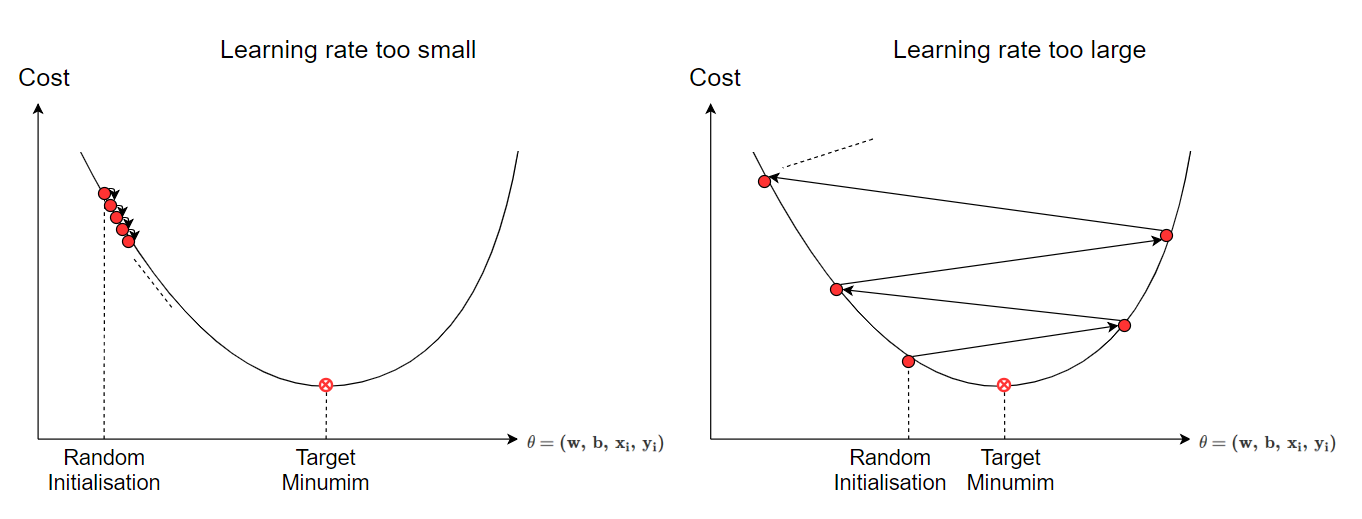
\includegraphics[scale = 0.5]{Images/learningrate.png}
  \caption{Gradient Descent behaviour depending on learning rate.}
  \label{learnrate}
\end{figure}



The backpropagation algorithm$^{\small \cite{backprop}}$ is now used to evaluate the partial derivatives, which can intuitively be interpreted as the gradient of the loss function, defined in the equations above. It starts from the final layer of the NN and computes the gradient directly from the loss function. Afterwards, it uses the chain rule to compute the gradient at each layer from the next layer until in reaches the input layer. \\



\subsubsection*{Predicting}

A trained model used on unseen data returns a prediction y. This can be used to estimate the class the input \textbf{x} lays in.

\begin{equation}
  c = \argmax_{c \in \{ c_1, c_2, ..., c_k\}} \ \mathbb{P}(\mathbf{x} \ \text{in class} \ c_i) = \argmax_{i \in \{ 1, 2, ..., k\}} \ y_i
\end{equation}

\smallskip

\section{Introduction to Patchy-San}

\section{Baseline Models}

This section briefly presents the theoretical background behind the classification models for which off-the-shelf implementations were used, serving as baselines for the context classification pipeline architecture. 

\subsection{K-Nearest Neighbours Classifier}
Many classification approaches attempt to estimate the conditional distribution of Y (output probabilities) given X (input features), and then classify a given observation to the class with highest estimated probability. One such method is the K-nearest neighbors (KNN) classifier$^{\small \cite{KNN}}$. Given a positive integer K and a test observation x$_0$, the KNN classifier first identifies the neighbours K points in the training data that are closest to x$_0$, represented by N$_0$. It then estimates the conditional probability for class $j$ as the fraction of points in N$_0$ whose response values equal $j$:

\begin{equation}
    Pr(Y = j|X = x_0) = \frac{1}{K} \sum_{i \in N_0} I(y_i = j)
\end{equation}

Finally, KNN applies Bayes rule and classifies the test observation x$_0$ to
the class with the largest probability. \\

In other words, KNN estimates how likely a data point is to be a member of one group or the other depending on what group the data points nearest to it are in. A worth noting aspect of KNN is that it is an example of a \textit{lazy learner} algorithm, meaning that it does not build a model using the training set until a query of the data set is performed, as opposed to the NN approaches later presented. \\




\subsection{Random Forest Classifier}

A decision tree$^{\small \cite{decision_tree}}$ is a classifier expressed as a recursive partition of the instance space. The decision tree consists of nodes that form a rooted tree. In a decision tree, each internal node splits the instance space into two or more sub-spaces according to a certain discrete function of the input attributes values. In the simplest and most frequent case each test considers a single attribute, such that the instance space is partitioned according to the attribute’s value. Each leaf is assigned to one class representing the most appropriate target value. Alternatively, the leaf may hold a probability vector indicating the probability of the target attribute having a certain value. Instances are classified by navigating them from the root of the tree down to a leaf, according to the outcome of the tests along the path. \\

Random forest classifier$^{\small \cite{RF}}$ creates a set of decision trees from randomly selected subset of training set. It then aggregates the votes from different decision trees to decide the final class of the test object. \\

\section{Requirement Analysis} \label{Requirement Analysis}

After performing an extensive inspection into the NN background theory, a decision was to be made regarding how to approach an implementation that satisfies the end goal of the project. Therefore, to build a ML pipeline capable of classifying, renaming and reorganising files in terms of both provenance and content information, a list of necessary steps is presented in Table \ref{Requirements overview}. \bigskip

\begin{longtable}{|p{.50\textwidth}|p{.15\textwidth}|p{.15\textwidth}|p{.15\textwidth}|}
  \hline
  \textbf{Requirements}                                        & \textbf{Priority} & \textbf{Risk} & \textbf{Difficulty} \\
  \hline
  Dataset understanding and investigation of existing patterns & High              & Low           & Low                 \\

  Receptive fields construction using Patchy-SAN               & High              & Low           & Medium              \\

  CNN implementation                                           & High              & Medium        & High                \\

  Generate synthetic data                                      & Medium            & Medium        & Medium              \\

  Hyperparameter tuning                                        & Medium            & Medium        & High                \\

  ML pipeline service time evaluation                          & Medium            & Medium        & Medium              \\

  Files renaming and reorganising implementation               & Low               & Medium        & Medium              \\

  \hline
  \caption[Requirements overview]{List of requirements for a successful project implementation, alongside with their risks and difficulties.}
  \label{Requirements overview}
\end{longtable} \bigskip


\section{Choice of Tools}

\subsection{Programming Languages}

I use Python 3.6.7 as the main programming language for building my project. This choice is sustained by the fact that Python provides an extensive selection of libraries and frameworks that facilitate deep learning algorithms implementation. Moreover, its syntax simplicity and high-quality documentation enhanced my experience throughout the development process. \\\

As a secondary programming language, I used Cypher Data Manipulation Language to interact with the original provided data set, which is stored as a graph database in Neo4J.

\subsection{Libraries}

The third-party libraries that were used alongside Python Standard Library are listed in Table \ref{Libraries}. \bigskip

\begin{longtable}{|p{.15\textwidth}|p{.10\textwidth}|p{.60\textwidth}|}
  \hline
  \textbf{Library} & \textbf{Version} & \textbf{Description}                                                                                                                                  \\
  \hline
  neo4j-driver     & 1.6.2            & Querying Neo4J graph database                                                                                                                         \\

  numpy            & 1.16.0           & Adds support for multi-dimensional arrays and matrices, along with a large collection of high-level mathematical functions to operate on these arrays \\

  sklearn          & 0.20.2           & Machine learning library                                                                                                                              \\

  networkx         & 2.2              & Used for for the creation, manipulation, and study of the structure, dynamics, and functions of complex networks                                      \\
  nauty            & 0.6.0            & Used for computing automorphism groups of graphs                                                                                                      \\

  matplotlib       & 3.0.2            & Data visualisation                                                                                                                                    \\


  \hline
  \caption[Libraries]{Third-party libraries used within project implementation.}
  \label{Libraries}
\end{longtable} \bigskip

\subsection{Development Environment}

Implementation, testing and evaluation of the project were performed on my personal machine (i7-6700HQ CPU 2.60GHz, 16GB RAM, 512GB SSD,  Ubuntu 18.04 LTS). Additionally, more resource intensive evaluations were carried out on GPUs provided by the Computer Laboratory Department. In terms of IDEs, I chose \textbf{PyCharm} due to its version control integration, on-the-fly error checking, debugging capabilities, flexibility and easy project navigation. \\\

To avoid possible issues created by either hardware/software failures or user errors, I had to place emphasis on adequately choosing backup strategies for my project. Thus, the git repository of the project was synchronised with \textbf{GitHub} online hosting service. The code was also occasionally updated on my Google Drive file space and on an external HDD. \\

\section{Starting Point}

I have started this project only having programming experience in C/C++ and Java. Thus, transition to Python was not problematic, as I had already covered fundamental concepts such as object-oriented and procedural programming. However, the more complicated stage was getting acquainted to the high-level NN APIs in Python. I needed to understand how to build NNs using off-the-shelf implementations for various layers, how to train, evaluate and optimise them. \\\

Moreover, I had only basic knowledge of machine learning. Part IA Machine Learning and Real World Data introduced the ideas of supervised learning and diverse evaluation metrics and strategies. However, additional preparation was needed to learn how NNs work, how to design their architecture, which regularisation techniques to use and what types would be most suitable for the project. \\

\section{Software Engineering Techniques}

Since all the requirements were clearly defined and understood, and also given the scale of the project, I decided to adopt the Iterative Development Model$^{\small \cite{iterative_model}}$. Respecting the concepts behind this software engineering model, I split my project into several modules that at first offer core functionality and are afterwards iteratively refined. The three indicated modules
consist of: database interaction module, machine learning pipeline module and a virtual filespace in which files are renamed and reorganised. \\\

Unit and integration testing were performed using (smaller) synthetically generated datasets. The datasets' generation tool gives the user full control over the way in which properties are generated and thus I could create similar patters to those in the original provenance graphs. \\

\section{Summary}

In this chapter, I introduced the neural networks background theory that supports the machine learning models built in the project, followed by analysing the requirements for achieving the success criteria and a brief description of the development environment and backup strategies. Furthermore, a software engineering model that describes how the project was step-by-step implemented and evaluated was also discussed. \\

\end{document}
\begin{document}

\chapter{Implementation}

In this chapter I will discuss how this project is structured, going through the high-level details of the actual implementation that respects all the requirements defined in Section \ref{Requirement Analysis}. It will review how the initial data is processed and how the extracted features of interest are used with a view to creating further synthetic and real datasets. Furthermore, the chapter examines how the Patchy-San algorithm operates on graph inputs in order to create suitable NNs training data and thus, how the NNs architectures are designed and optimised for the given classification task. Finally, the way in which files are renamed and reorganised into a virtual filesystem are analysed. \\


\section{Data Analysis and Processing}

\subsection{Data Properties}

\begin{figure}[H]
  \centering
  \centerline{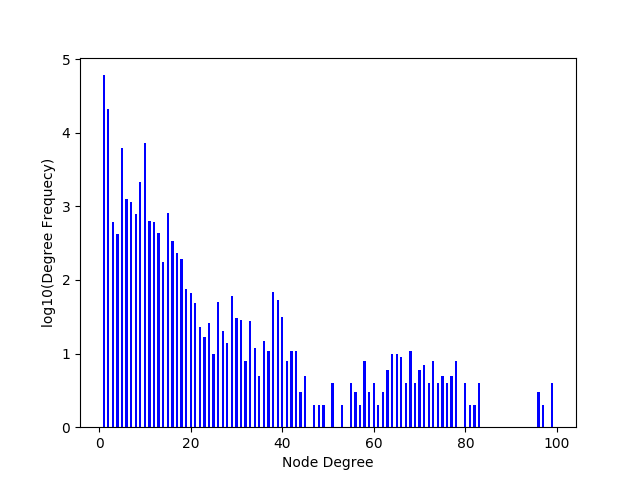
\includegraphics[scale = 0.86]{Images/nodedegdist.png}}
  \caption{Node degree distribution in Neo4J database.}
  \label{nodedegdist}
\end{figure}

\subsection{Neo4J Interaction and Feature Extraction}

\subsection{Feature Engineering}

\subsection{Synthetic Data Generation} \label{synthetic data generation}


\section{Overall Structure of the Project}

\begin{figure}[H]
  \centering
  \centerline{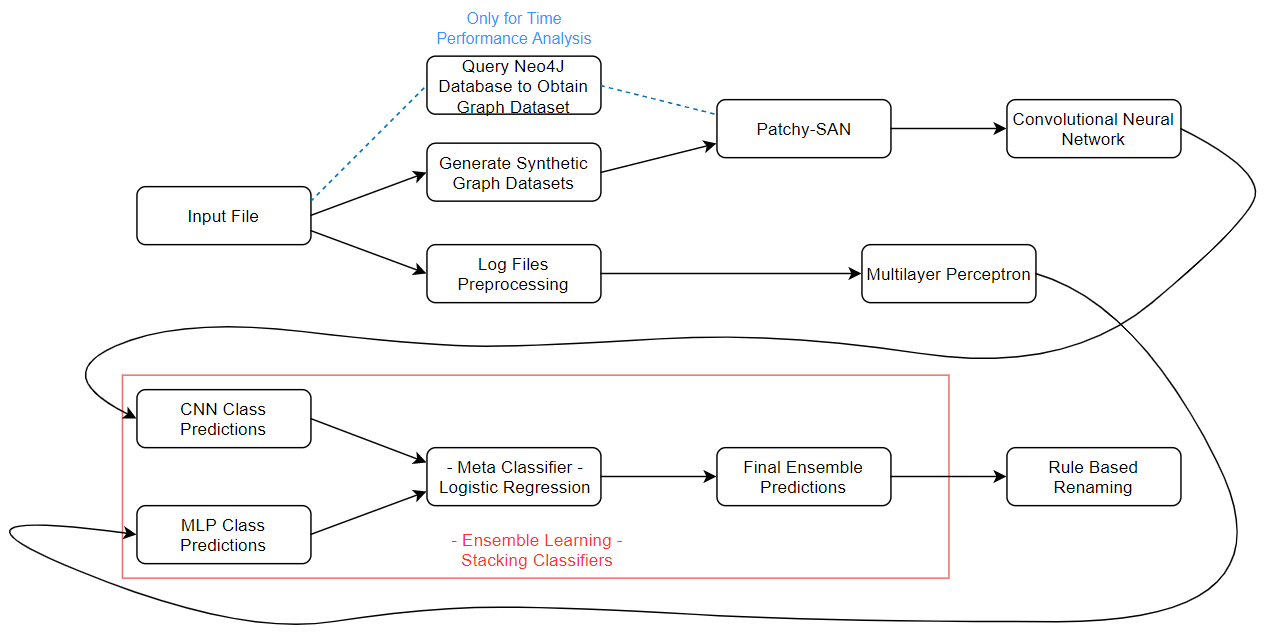
\includegraphics[scale = 0.6]{Images/pipeline.png}}
  \caption{Overview of the implemented ML pipeline.}
  \label{pipeline}
\end{figure}

\begin{figure}[H]
  \centering
  \centerline{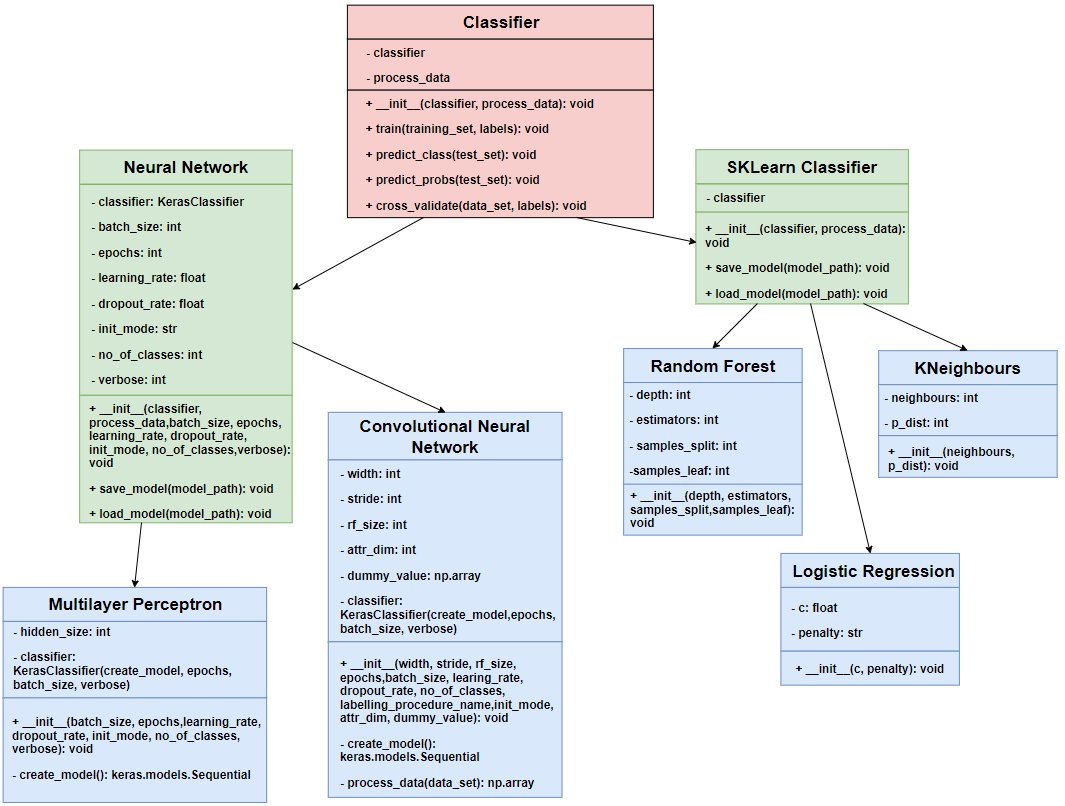
\includegraphics[scale = 0.7]{Images/uml.png}}
  \caption{UML diagram illustrating the inheritance of implemented classifiers.}
  \label{OOP}
\end{figure}

\subsection{Overview of the Renaming Pipeline}

\subsection{Nested Cross-Validation}

The fundamental success criteria of the project were to develop, tune and evaluate a ML pipeline capable of classifying files in term of both content and provenance graph. In order to deal with the second and third mentioned goals, I have implemented a Nested Cross-Validation (CV) procedure. A detailed description of how it is performed follows and an expressive visualisation of it can be observed in Figure \ref{NestedCV}. \bigskip

\begin{itemize}[label={}]
  \item 1. divide the dataset into K stratified cross-validation folds at random
  \item 2. for each fold $k$ = 1,2,...,K (outer loop for evaluation of the model with selected hyperparameter):
        \begin{itemize}[label={}]
          \item 2.1. let fold $k$ be the outer test set
          \item 2.2. let all data except for fold $k$ be the outer training set
          \item 2.3. randomly split training set into L stratified fold
          \item 2.4. for each fold $l$ = 1,2,...,L (inner loop for hyperparameter tuning):
                \begin{itemize}[label={}]
                  \item 2.4.1. let fold $l$ be the inner validation set
                  \item 2.4.2. let all data except fold $k$ and fold $l$ be the inner training set
                  \item 2.4.3. train with each hyperparameter on inner training set and evaluate on fold $l$, keeping track of performance metrics
                \end{itemize}
          \item 2.5. for each hyperparameter setting, calculate average metrics score over the L folds and choose the best one
          \item 2.6. train a model with the best hyperparameter on fold $k$, evaluate its performance and save its score
        \end{itemize}
  \item 3. calculate the mean score over all K folds and report as the generalisation error
\end{itemize} \bigskip

An outer CV procedure is performed to provide a performance estimate used to select the optimal model. In each fold of the outer CV, the hyperparameters of the model are tuned independently to maximise an inner CV estimate of generalisation performance. The outer CV is then essentially estimating the performance of a method for fitting a model, CV based hyperparameter tuning. This eliminates the bias introduced by a flat CV procedure as the test data in each iteration of the outer CV has not been used to optimise the performance of the model in any way, and may therefore provide a more reliable criterion for choosing the best model. Another advantage consists of tuning and evaluating on the entire dataset, instead of completely discarding the validation set. The computational expense of nested CV, however, is substantially higher. \\



\begin{figure}[H]
  \centering
  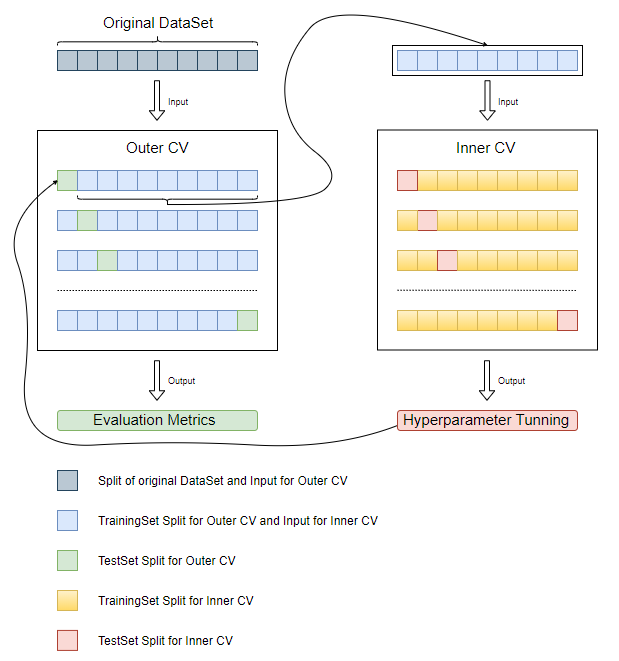
\includegraphics[scale=0.95]{Images/nested_cv.png}
  \caption{Structure of a Nested Cross-Validation used for both model evaluation and hyperparameter tuning.}
  \label{NestedCV}
\end{figure}


\section{Patchy-San}

Patchy-San aims to bring CNNs to bear on a large-class of graph based learning problems. This novel algorithm consists of a general approach of extracting locally connected regions from graphs and model them in such a way so that they become a suitable input for a CNN. In this context, suitable refers to both structurally adequate and having the capability of preserving graph's expressivity, in the sense that local pattern information is not lost when linearising the set of features. \\

My re-implementation brings a few adjustments and extensions (mentioned in the upcoming sections) to the original algorithm so that it suits better the shape and properties of the dataset provided. \\

\subsection{Node Sequence Selection}

The first step in the algorithm consists of establishing a node ordering for the input graph based on a chosen graph labelling function. In general, any reasonable graph labelling function would work for this sorting procedure. For instance, an artificial, independent of dataset knowledge approach, can use the betweenness centrality value of each node. However, given the insights into the provenance dataset, I chose to use the timestamp of the influence relations for labelling purposes, as this would imply a more natural ordering and actually improve the overall results. \\

Given this ordering, a subset of nodes is designated as the roots (Node Sequence) from where the actual receptive fields will be constructed. Specifically, each two consecutive picked roots from the sorted list of nodes are within a constant distance from each other. This distance ($s$) is called a stride. The aim is to construct the same $w$ number of receptive fields for each input graph as they will be provided as training/testing data for the convolutional neural network. Therefore, in case the number of nodes is not sufficient for building $w$ receptive fields, the algorithm creates all-zero receptive fields for padding purposes. \\

\begin{figure}[H]
  \centering
  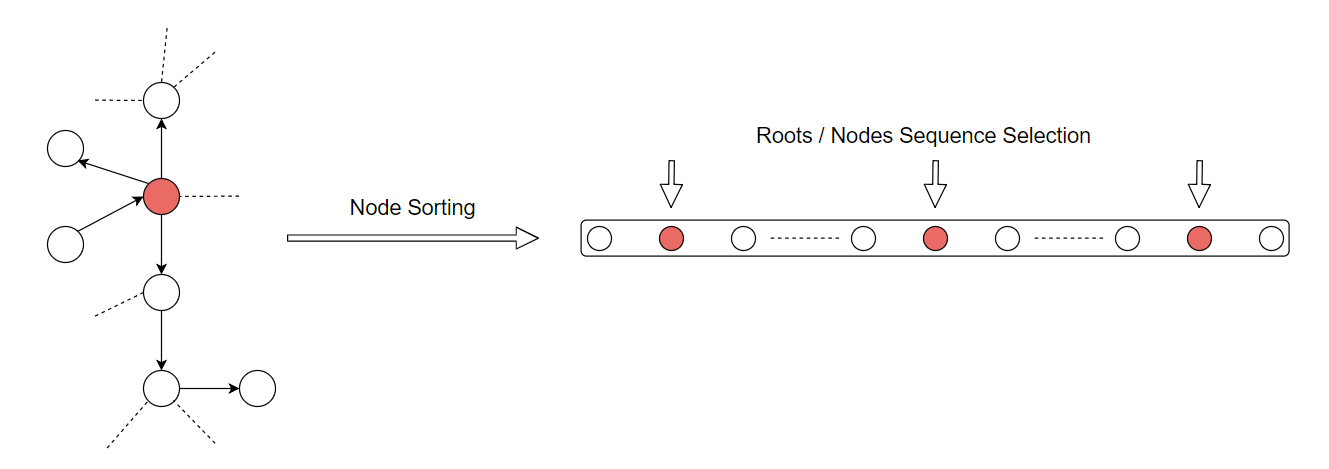
\includegraphics[scale=0.5]{Images/nodeseqsel.png}
  \caption{Input graph node's sorted with respect to the labelling function. $w$ root nodes selected within stride $s$.}
  \label{nodeseqsel}
\end{figure}

\subsection{Neighbourhood Assembly}

The next stage involves assembling a local neighbourhood for each root previously determined. This is accomplished by using a standard breath-first search algorithm. Thus, I explore vertices with an increasing distance from the root, adding them to a set N. If the number of collected nodes is smaller than a pre-established number $k$, I continue exploring the immediate neighbours of the latest nodes added to the set until either $k$ nodes are found, or there are no more neighbours. In the latter case, for padding purposes, dummy nodes, having dummy attributes are added. This helps not throwing away information that might convey in-graph patters. However, it introduces the risk of misidentifying the padding nodes as a pattern themselves. \\

One final remark for the neighbourhood assembly procedure is that the order in which the immediate neighbours of a node are explored is with respect to, once again, the timestamp of each influence edge. Specifically, newer system activities will be considered with priority, also ensuring that the procedure is consistent and always gives the same output for the same graph. \\

\begin{figure}[H]
  \centering
  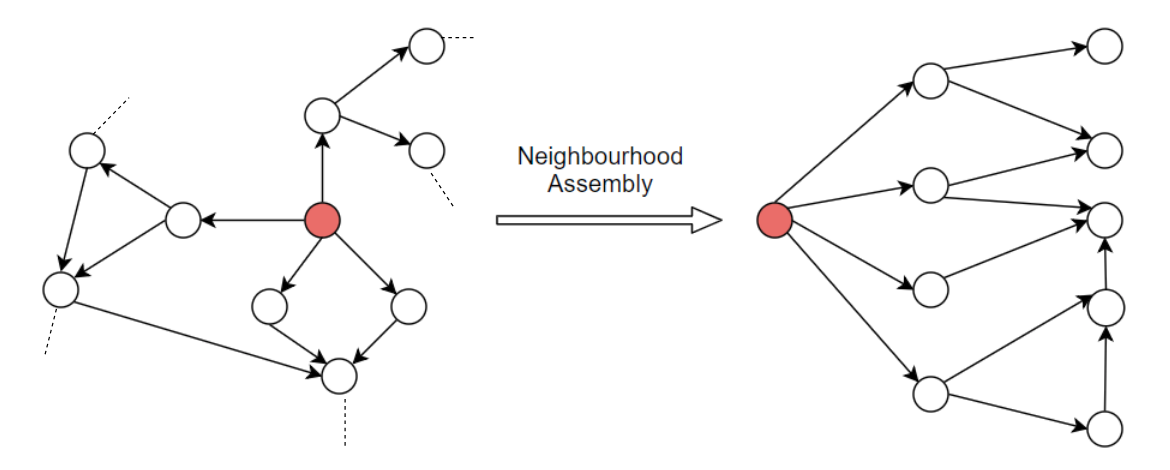
\includegraphics[scale=0.375]{Images/neighassemb2.png}
  \caption{Illustration of a Breath-First Search used for computing a neighbourhood.}
  \label{neighassemb}
\end{figure}


\subsection{Receptive Field Normalisation}

The receptive field of a node is built by normalising the neighbourhood assembled in the previous step. The normalisation imposes an order on the nodes of the neighbourhood graph so as to map from the unordered graph space to a vector space with a linear order. This time, the graph labelling procedure is way more difficult to compute, as appropriately choosing it is at the core of the representation that Patchy-San proposes. Hence the performance of the classification pipeline will highly depend on the labelling procedure. \\

The basic idea is that the graph labelling procedure should assign nodes of two different graphs in similar positions if and only if they have similar structural roles in the graphs. The labelling of the vertices is therefore constrained by the graph distance to the root node $v$. For any two vertices $u$, $w$, if $u$ is closer to $v$ than $w$, then $v$ is
always ranked higher than $w$. This definition, illustrated in Figure \ref{normalisation}, ensures that $v$ has always rank 1, and that the closer a vertex is to $v$ in the graph, the higher it is ranked in the vector space representation. Consequently, in my project, this implies that groups of nodes denoting: processes interacting directly with the file to be classified, parent processes of the ones just mentioned, past processes interacting with the file at different moments in time; will be close together in the linear representation and also in same order for different graphs.\\

\begin{figure}[H]
  \centering
  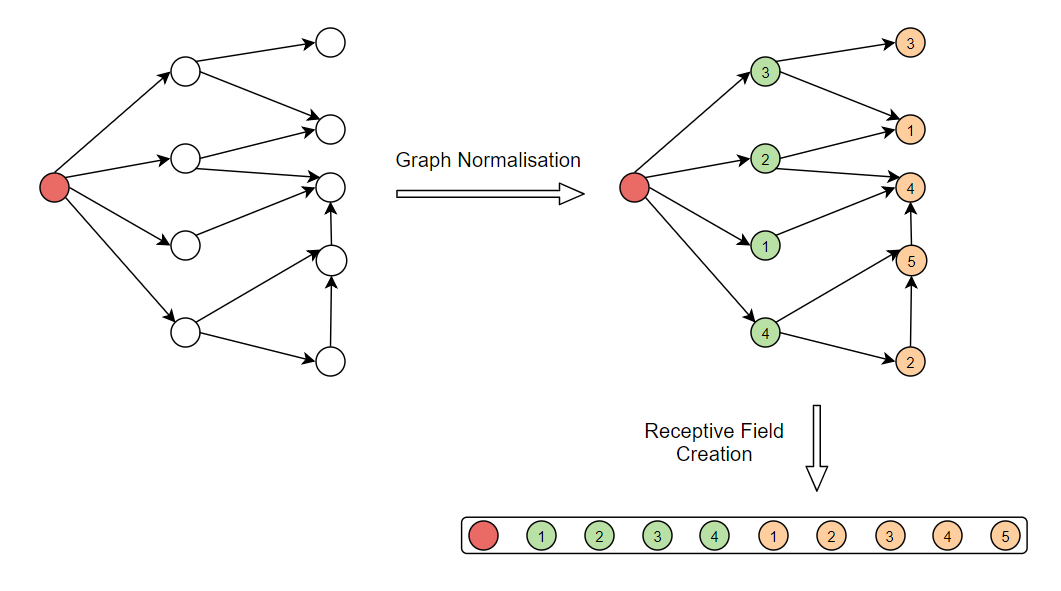
\includegraphics[scale=0.55]{Images/normalisation.png}
  \caption{Receptive Field Normalisation from previously selected neighbourhood. Nodes having the same colour have the same rank with respect to root in the liniarisation, while numbers illustrate tie-breakers.}
  \label{normalisation}
\end{figure}

One important detail that was taken into account is that, in general, the described labelling procedure does not consist of an injective function, thus a method to break ties between same-labelled nodes is necessary.

\section{Convolutional Neural Network}

For each input graph $G$, given the construction of the receptive fields, and the number of attributes of each vertex $a_v$, I compute an initial 3D tensor of sizes ($w$, $k$, $a_v$), which is afterwards reshaped to a 2D tensor ($wk$, $a_v$) and fed as input for the CNN (where, obviously, $a_v$ will be the number of input channels). \\

\subsection{Parameter initialisation}

The initial values of the parameters of a NN drastically influence the quality of the solution returned by the mini batch gradient descent optimisation algorithm, as they may direct the process towards different local minima. NN's weights receive an update proportional to the partial derivative of the error function with respect to the current weight in each iteration of training. Therefore, if the initial weights are too small, they will shrink exponentially as they go deeper and deeper into the network, until they vanish. This situation severely reduces NN's capacity of representing non-linearities. On the other hand, if the initial weights are too large, they will grow exponentially larger as they go deeper and deeper into the network, until they might overflow, crashing the model. Even if the parameters don't overflow, the layers can still become insanely large, resulting in the algorithm diverging. Bearing these two aspects in mind, the aim is to distribute the initial parameters in such a manner that they can successfully (i.e. not vanishing nor exploding) travel forwards and backwards withing the network. \\

The initialisation strategy used for the CNN is He initialisation and consists of ...\\

The initialisation strategy used for the MLP is called Xavier initialisation. It takes into account the problems shown above and bases the standard deviation or the variance of the weight initialisation on the number of variables involved. It thereby adjusts itself based on the number of weight values. It works on the idea that if the variance is kept constant from layer to layer in both the feed forward direction and back-propagation direction, the network will learn optimally. Specifically, this method initialises weights by drawing them from a small Gaussian distribution with: \\

\begin{equation}
  \centering
  \mu = 0 \ \text{and} \ \sigma^2 = \frac{2}{n_{in}}
\end{equation}

where $n_{in}$ is the number of neurons which serve as input for the layer to which the weight belongs. \\

\begin{figure}[H]
  \centering
  \centerline{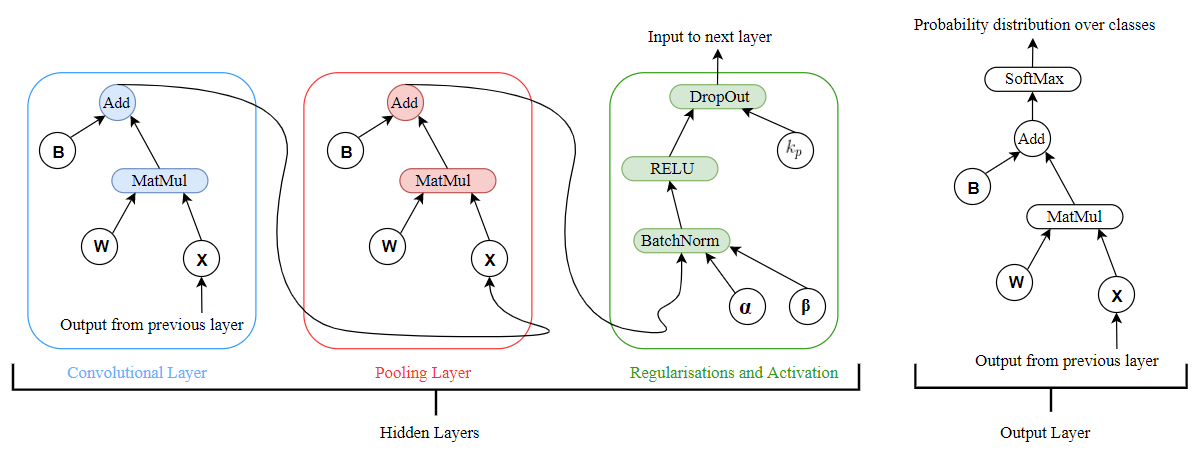
\includegraphics[scale=0.6]{Images/cnn_layers.png}}
  \caption{Diagram illustrating the configuration of hidden and output layers of the CNN.}
  \label{cnn_layers}
\end{figure}

     \begin{figure}[H]
  \centering
  \centerline{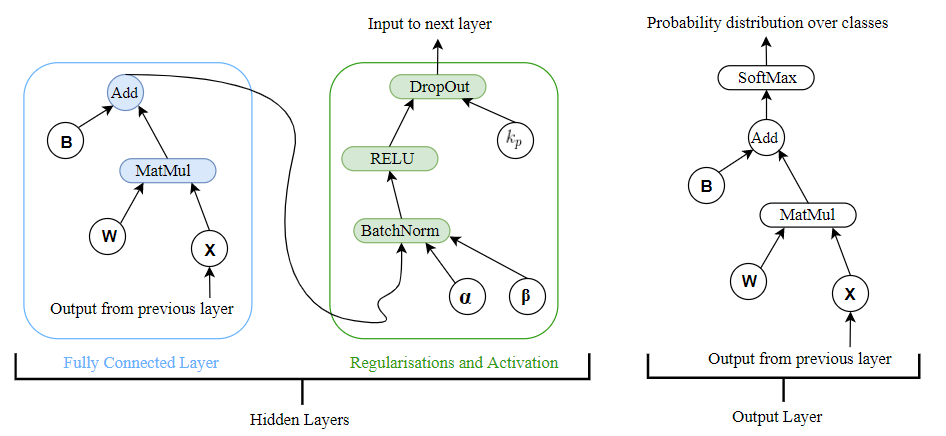
\includegraphics[scale=0.6]{Images/mlp_layers.png}}
  \caption{Diagram illustrating the configuration of hidden and output layers of the MLP.}
  \label{mlp_layers}
    \end{figure}

\section{Regularisation Techniques}

Deep NNs can be trained to develop complex relationships between their input data and their outcome. Depending on the amount of training data the network may develop a behaviour that brings good results for the training data, but fails as soon as unknown test data is fed into the network. To prevent overfitting in neural networks, there exist a variety of methods. A few of them were implemented and are discussed in this section.

\subsection{Dropout}

Dropout is a regularisation technique behaving in the following manner: on each training iteration, a randomly chosen subset of neurons in the NN are shut down, in the sense that the NN will perform forward propagation and back-propagation as if those nodes (alongside with their inwards and outwards edges) are not preset at all. Since the units that are dropped out in each iteration are random, this forces the learning algorithm to spread out the weights and not focus on some specific features. This procedure can be visualised in Figure \ref{dropout}. In the simplest case, each unit is retained with a fixed probability $p$ independent of other units, which is introduced as a new hyperparameter in the NN. \\

One important aspect to note is that the weights of the network will be larger than normal because of dropout. Thus, if a unit is retained with probability $k_p$ during training, the outgoing weights of that unit are multiplied by $p$ at test
time. Another approach is to re-scale weights at training time instead, after each weight update at the end of the mini-batch. This is sometimes called inverse dropout and is the way both Keras and Pytorch deep learning libraries implement it. \\


\begin{figure}[H]
  \centering
  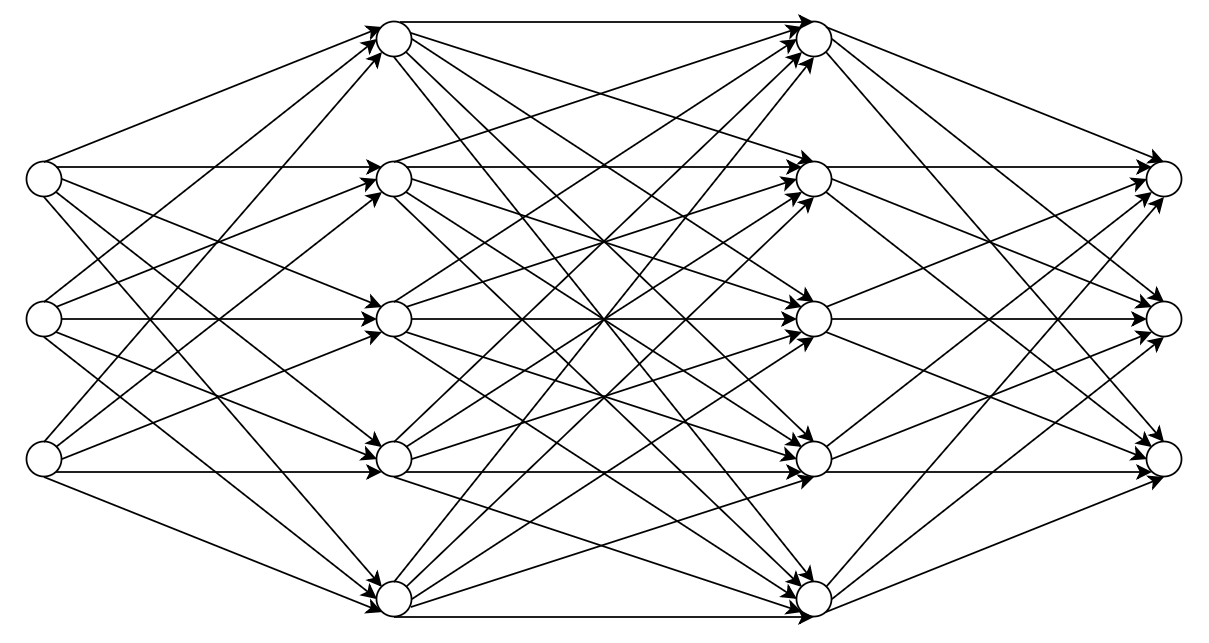
\includegraphics[scale=0.35]{Images/beforedrp.png}

  \bigskip

  \bigskip

  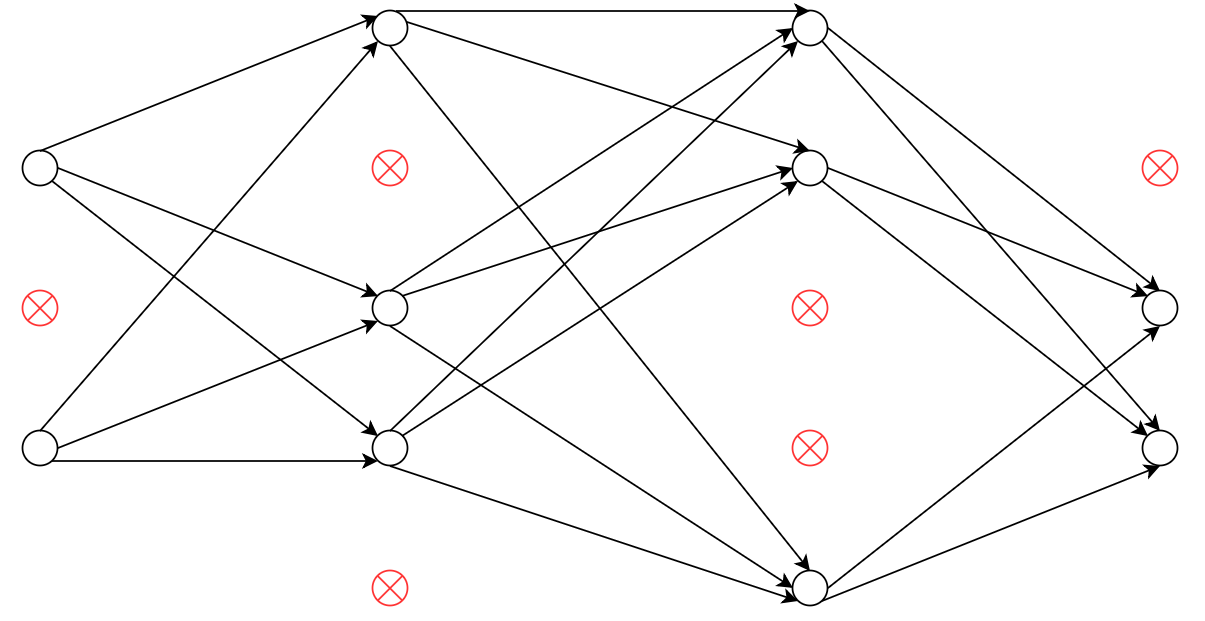
\includegraphics[scale=0.35]{Images/afterdrp.png}

  \bigskip

  \caption{Neural Network before (upper image) and after (lower image) dropout.}
  \label{dropout}
\end{figure}

\subsection{Batch Normalisation}


One of the key motivations for the development of Batch Normalisation was the reduction of so-called internal covariate shift (ICS). ICS is the phenomenon wherein the distribution of inputs to a layer in the NN changes due to an update of parameters in the previous layers. This change leads to a constant shift of the underlying training problem and is thus believe to have detrimental effect on the training process. \\

Therefore, Batch Normalisation is a mechanism that aims to stabilise the distribution (over a mini-batch) of inputs \{$x_1$, $x_2$, ... , $x_n$\} to a given NN during training. This is achieved by augmenting the NN with additional layers that set the first two moments: mean - $\mu = \frac{1}{n} \sum_{i=1}^n x_i$ and variance - $\sigma = \sqrt{\frac{1}{n} \sum_{i=1}^n (x_i - \mu) ^ 2}$, of the distribution of each activation to be zero and one respectively. Thus, it normalises the inputs in the following manner: \\

\begin{equation}
  \centering
  \hat{x}_k = \frac{x_k - \mu}{\sqrt{\sigma + \epsilon}}
\end{equation}

where $\epsilon > 0$ is a small constant added to avoid division by 0. \\

Then, the batch normalised inputs are also typically scaled and shifted based on trainable parameters $\gamma$ and $\beta$ to preserve model expressivity. \\

\begin{equation}
  \centering
  y_k = \gamma_k * \hat{x}_k + \beta_k
\end{equation}

\subsection{Weight Decay}
Weight decay is a standard trick to improve the generalisation performance of neural
networks by constraining the weights to be small in magnitude and penalizing large weights. Specifically, weight decay is defined as multiplying each weight in the gradient descent at each epoch by a factor $\lambda$ smaller than one and greater than zero. This technique is equivalent to introducing an L2 regularisation term to the loss function that one wants to optimise. Therefore, the updated loss functions will be of the following form: \\

\begin{equation}
  \centering
  \mathfrak{L}_{updated} = \mathfrak{L}_{model} + \frac{\lambda}{2} \norm{\textbf{w}}
\end{equation}

where $\norm{\textbf{w}} = \sqrt{\sum |w_i^2|}$ is the L2 norm of the weights vector.\\

Keras provides a weight regularisation API that allows one to add a penalty for weight size to the loss function. A weight regularizer can be added to each layer when the layer is defined in a Keras model. This is achieved by setting the $kernel\_regularizer$ argument on each layer.

\subsection{Early Stopping}
A problem with training neural networks is in the choice of the number of training epochs to use. Too many epochs can lead to overfitting of the training dataset as well as high training times, whereas too few may result in an underfit model. Early stopping is a method that allows one to specify an arbitrary large number of training epochs and stop training once the model performance stops improving on a hold out validation dataset. The error on the validation set is used as a proxy for the generalisation error in determining when overfitting has begun (i.e. the moment that after achieving a minimum, the error on the validation set starts increasing again).\\

Keras supports the early stopping of training via a callback called EarlyStopping. This callback requires setting the performance measure to monitor (hence defining what is considered to be an improvement), the trigger, and once triggered, it will stop the training process. In Keras, callbacks provide a way to execute code and interact with the training model process automatically. Callbacks can be provided to the \textit{fit()} function via the \textit{callbacks} argument. Often, the first sign of no further improvement may not be the best time to stop training. This is because the model may coast into a plateau of no improvement or even get slightly worse before improving considerably. We can account for this by adding a delay to the trigger in terms of the number of epochs on which we would like to see no improvement. This can be done by setting the \textit{patience} argument. \\


\section{Renaming the Files}

\section{Building a Virtual File System}


\section{Summary}


\end{document}
\begin{document}

    \chapter{Evaluation}
    
    \section{Success Criteria}
    
    The initial success criteria for a core implementation of the project were defined in the original Project Proposal and are listed below: \\
    
    \begin{itemize}
        \item \textit{develop and optimise a machine learning pipeline that can use both provenance data and content data in order to do the file classification}. \\
        
        \item \textit{perform a quantitative evaluation of the implemented architecture(s) and investigate the best trade-off of precision and recall}. \\ 
        
        \item \textit{investigate the performance of the implemented pipeline in terms of time and space requirements}. \\
        
    \end{itemize}
    
    
    \section{Evaluation Methodology}
    
    \subsection{Classification Metrics}
    
    \subsubsection*{Metrics for Binary Classification}
    
    A confusion matrix for binary classification consists of a 2 by 2 table which reports the number of true positives (TP), true negatives (TN), false positives (FP) and false negatives (FN). The confusion matrix can be regarded as a technique for summarising the performance of a classification algorithm, as all the metrics used for evaluation are derived from it. 
    
    \begin{figure}[H]
        \centering
        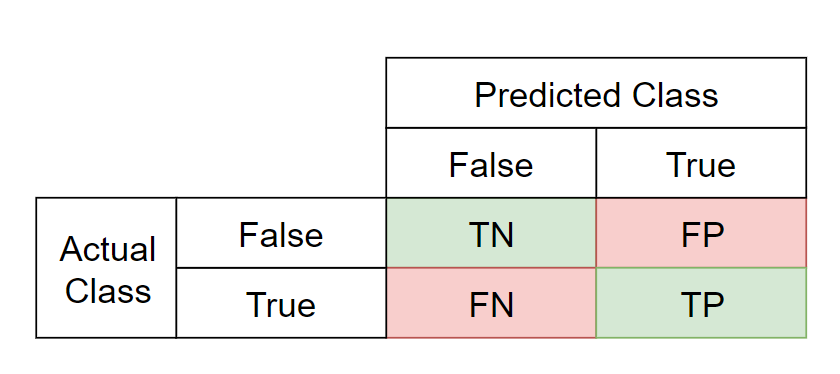
\includegraphics[scale = 0.4]{Images/2dconfusion.png}
        \caption{Confusion matrix for 2 classes.}
        \label{2classmatrix}
    \end{figure}
    
    Therefore, the most common metrics are: \\
    
    \begin{itemize}
        \item \textbf{Accuracy} (what \% of predictions were correct): $$ \cfrac{\text{number of corect predictions}}{\text{total number of predictions made}} = \cfrac{TP + TN}{TP + TN + FP + FN}$$ \\
        Probably the most straightforward and intuitive metric for classifier performance. However, it is misleading when confronted with class imbalance problem. \\
        
        \item \textbf{Precision} (what \% of positive predictions were correct): $$ \cfrac{TP}{TP + FP}$$ 
        In the context of fraud detection, it is usually more costly to miss a positive instance than to falsely label a negative instance. Hence, we are concerned with precision rather than recall. \\
        
        \item \textbf{Recall} (what \% of positive cases did model catch): $$ \cfrac{TP}{TP + FN}$$ \\
        In situations where you want to detect instances of a minority class, you are usually concerned more with recall than precision. \\
        
        \item \textbf{F1 score} (weighted average of precision and recall): $$ \cfrac{2(\text{precision} \ * \ \text{recall})}{\text{precision} \ + \ \text{recall}} = \cfrac{2TP}{2TP + FP + FN}$$ \\
        As all of the metrics above, F1 score takes values between 0 and 1, higher values indicating better performance. In fact, higher values of F1 score indicate better balance between precision and recall. \\ 
        
        \item \textbf{Matthew's Correlation Coefficient (MCC)} $$ \cfrac{TP * TN + FP * FN}{\sqrt{(TP + FP)(TP + FN)(TN + FP)(TN + FN)}}$$ \\
        Unlike the other metrics discussed above, MCC takes all the cells of the Confusion Matrix into consideration in its formula, hence behaves the best in case of imbalanced classes. The range of values of MCC lie between -1 to +1. A model with a score of +1 is a perfect model and -1 is a poor model, while a score of 0 is a as good as a random model. This property is one of the key usefulness of MCC as it leads to easy interpretability. \\
    \end{itemize}
    
    \subsubsection*{Metrics for MultiClass Classification}
    
    In order to extend the 2D confusion matrix for the general case, I will adopt a One-vs-All (OVA) classifiers approach which reduces the problem to binary classification. Specifically, each class will be in turn considered the positive/true class, while all the others merged will be the negative/false class. At each step, the metrics described in the previous subsection will be computed and afterwards combined in a couple of different ways to form their variations used for evaluating multiclass classification. \\
    
    \begin{figure}[H]
        \centering
        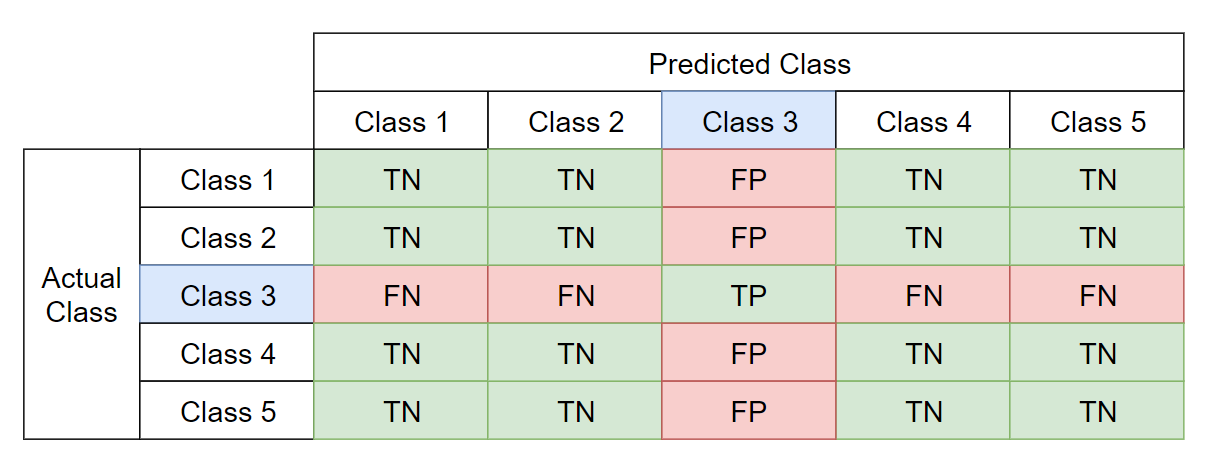
\includegraphics[scale = 0.5]{Images/5dconfusion.png}
        \caption{Confusion matrix for multiple classes using OVA approach where Class 3 is the positive class.}
        \label{5classmatrix}
    \end{figure}
    
    Let TP$_i$, TN$_i$, FP$_i$, FN$_i$ be the number of true positives, true negatives, false positives and false negatives when class $i$ is regarded as the positive class. Moreover, let Metric$_i$ be the value of an evaluation metric when class $i$ is regarded as the positive class, where Metric is one of Precision, Recall, F1 score, MCC (note that Accuracy can be computed as before i.e. $ \frac{\text{number of corect predictions}}{\text{total number of predictions made}}$). Thus, Metric$_i$ is computed using TP$_i$, TN$_i$, FP$_i$, FN$_i$ as inputs. Given these definitions, there are two approaches to average the class specific metrics in order to obtain the metrics used for evaluating multiclass classifiers: \\
    
    \begin{itemize}
        \item \textbf{Micro Averaging}: \\
            Micro-Multiclass-Metric = Metric($\sum_{i=1}^{N}$ TP$_i$, $\sum_{i=1}^{N}$ TN$_i$, $\sum_{i=1}^{N}$ FP$_i$, $\sum_{i=1}^{N}$ FN$_i$) \\
             A micro-average will aggregate the contributions of all classes to compute the average metric. In a multi-class classification setup, micro-average is preferable when we suspect there might be class imbalance.
            
        \item \textbf{Macro Averaging}: \\
            Macro-Multiclass-Metric = $\cfrac{1}{N}$ $\sum_{i=1}^{N}$ Metric$_i$ \\
            A macro-average will compute the metric independently for each class and then take the average (hence treating all classes equally).
    \end{itemize}
    
    
    
    \subsection{Monte Carlo Permutation Test}
    
    In order to comparatively evaluate any two models implemented, I use the \textbf{permutation} \textbf{test} for paired samples. The permutation test checks whether the population mean of the two conditions is different (H$_1$) or the same (H$_0$). The power of the permutation test is defined as 1 - $\alpha$ where: 
    
    \begin{equation}
        \centering
        \alpha = \mathbb{P}(\text{Do not reject H$^0$ | H$_1$ is true}) \newline
    \end{equation}    
    i.e. the test declares no difference, where there really is one. \\
    
    I opted for the permutation test as it is known to have higher power than the, perhaps more popular, sign test \cite{signtest}. The core assumption of the permutation test is that if the measured difference \textit{d} in mean M between systems A and B is a fluke, i.e., if there is no real difference between them (because they come from one and the same distribution), it should not matter how many times one randomly swaps the two results. Consider \textit{n} paired results of System A and B. There are 2$^n$ ways of flipping or not flipping the n pairs of results, i.e., 2$^n$ permutations. These permutations operate row-wise. In other words, we create resamplings of these permutations in the following way: for each paired observation in the original runs, $a_i$ and $b_i$, a coin is flipped. If it comes up heads, then swap the score for $b_i$ with $a_i$. Otherwise, leave the pair unchanged. Now calculate the means M of the two system under this permutation, calculate their difference in means, and then do it 2$^n$ times for all permutations. Count how many of the 2$^n$ differences are as high as the difference in the unpermuted version. Call this number S. \\
    
    Finally, if due to a high number \textit{n} you cannot do all exponentially many resamplings, then a large enough random subset of cardinality R should be tested. This version of the test is called \textbf{Monte Carlo Permutation Test}. The probability of observing the difference between the original runs by chance approximated by: \\
    
    \begin{equation}
        p = \cfrac{S + 1}{R + 1}
    \end{equation}

    \smallskip
    
    I decide that two sets of predictions come from different distributions for p-value $\leq$ 0.05 and I choose R = 5000.
    
    \subsection{ML Pipeline Time and Space Performance Metrics}
    
    \section{Evaluation Results and Discussions} \label{Evaluation Results}
    
    \section{Summary}
    
\end{document}
\begin{document}
    
    \chapter{Conclusions}
    This dissertation presented the effort put in designing, implementing, tuning and evaluating a machine learning pipeline capable of combining both provenance data and content information in order to classify and rename files.
    
    \section{Achievements}
    All the success criteria of this project have been achieved and exceeded. The results obtained with respect to the metrics established in the Evaluation section are promising. They conceptually prove that NNs can constitute a great approach when it comes to dealing with both graph and file content classifications.  Moreover, the comparative analysis performed in Section \ref{Evaluation Results} gave an excellent perspective on the performance of the different models implemented. The challenge raised by the sparsity of the dataset provided was also well overcome by generating appropriate synthetic datasets.
    
    
    \section{Lessons Learnt}
    It goes without saying that the theoretical knowledge that I had to familiarise myself with is of paramount importance in the field of Machine Learning. This was a topic that aroused my interest throughout the project, especially how algorithms can be deployed such that they replicate human-like capabilities. Hence, successfully completing it brought myself a lot of satisfaction. \\
    
    However, I would like to highlight the experience gained in designing neural networks, as I have discovered that this is comprised of multiple stages, perhaps each equally important. It starts with a challenging data processing and feature engineering step, that might require very complex algorithms such as Patchy-San which transforms raw graphs into suitable input for NNs. It continues with an iterative process of choosing an actual architecture for a NN, tuning hyperparamenters and applying various regularisation techniques. All of these become especially difficult as there is no given recipe which works under every circumstances. Each task is different in itself and requires time and inspection of different strategies on all the described stages. \\
    
    If I were to start the project again, I would have allowed more time on the content side of the pipeline. I would have tried to explore how to design appropriate features for different types of files, and respectively, on other methods of combining them with features extracted from the provenance graphs. \\ 
    
    \section{Further Work}
    
    Working on this project was an invaluable practice from the perspective of a future computer scientist, still inexperienced in the software development field. Although strong results were achieved, there is still space for very intriguing questions. With a view to answering some of them, the following further extensions could be implemented:
    
    \begin{itemize}
        \item \textit{Exploring different NN architectures}: many novel architectures such as Graph Attention Networks$^{\small \cite{GAT}}$, Graph Convolutional Networks$^{\small \cite{DGCNN}}$ and Variational Recurrent Networks$^{\small \cite{RNN}}$ have shown promising results in the research field. It would make a great extension running a comparative between some of them and the Patchy-San-CNN pipeline.
        
        \item \textit{Evaluate the context classification algorithm on real data}: check whether the L2$_{distance}$ assumption when generating the node properties' distributions does actually match real data properties. 
        
        \item \textit{Implement ML models that can predict user's renaming strategies:} go a step further then doing standard rule-based renaming. A ML model could perhaps learn the methods in which a user chooses to rename the files and relate them to the currently obtained classification.    
    
    \end{itemize}
    
\end{document}
\appendix
% 
\begin{document}

\chapter{Project Proposal}
\begin{center}
  \Large
  Computer Science Tripos -- Part II -- Project Proposal\\[4mm]
  \LARGE
  Descriptive file names from content and context \\[4mm]

  \large
  Tiberiu-George Copaciu, Homerton College

  Originator: Dr Lucian Carata

  19$^{th}$ October 2018
\end{center}

\vspace{5mm}

\textbf{Project Supervisor:} Dr Lucian Carata

\textbf{Director of Studies:} Dr John Fawcett

\textbf{Project Overseers:} Dr Simone Teufel  \& Dr Andrew Rice

% Main document

\section*{Introduction}

\subsubsection*{Description}

This project addresses the problem of files that are created either by users or by processes among which many of them end up having extremely unintuitive or non-descriptive names (e.g. foo, bar, stdin, stdout). Specifically, based on the contents of the file and the context within which it was created the project aims to classify and rename/reorganize files by providing users with a virtual view of the file system. This view (a virtual file system) is built based on both the classification and user-given policy.

\subsubsection*{Dataset}

The target dataset consists of system traces taken from machines on which typical developer/attacker behaviour and work-flows are simulated. Furthermore, the data is synthetically generated to mimic real activity (i.e. it is not a simple script to repeat things in a loop), with attacks performed by a "red team" (i.e. a team specialised in attacking systems) as part of a DARPA project on Transparent Computing. \\
In terms of the format of the data I will be working with, these traces are already converted into a graph database according to a well defined model called OPUS/PVM (\url{https://www.cl.cam.ac.uk/research/dtg/fresco/opus}). In the mentioned graphs the nodes represent precesses, files, sockets and other system-level entities, while the edges represent influences and data-flow. The target files can be human-written documents, but most would be outputs generated by various programs and processing pipelines. \\
Unintuitive or non-descriptive names (i.e. the main concern of the project) can be the result of several actions either intentional (e.g. different names created by attackers to disguise the actual content of a file/document before exfiltration) or something that appears organically as part of the using system (e.g. results from running of scripts and experiments that use temporary file names which are not deleted; produced by the simulated developers while downloading documentation from the Internet).

In terms of privacy, although everything is made to look similar to real user behaviour, these traces are not genuine activities and no sensitive data is involved. The traces will be made public, hence there is no expectation of privacy. Similar techniques like those used in this project can perhaps be applied on real users and documents, but this has much tougher privacy/ethics implications. \\


\subsubsection*{Overview}

The first part of the project consists of classifying the files into appropriate categories using machine learning techniques. The machine learning model(s) used will have to take into account both the structure/content of the files and the structure of the graph(i.e. the context in which the file is used or was created). With regards to the context, it refers to a full provenance graph, rather then just to the program that created the file or the user that writes to the file. The second part of the project implies implementing the re-naming of files based on user-given policy and on-the-fly. Also, another target is to determine a more intuitive organization of the files in the file system, taking into account the obtained classification. Furthermore, the project will present the user a virtual file system in which the files appear with different names and possibly in a different hierarchy (rather than directly making changes to them). \\


\subsubsection*{Machine Learning Motivation}

The point of the project is to explore how/with what degree of success can machine learning be deployed to deal with the naming/structuring issues mentioned above. It is true that there is less variation in the data than a human running a system over a long period of time, and in that sense the problem is simpler. However, not applying machine learning means one has to know a lot more about what executes on the system and the types of files or the types of activity that generates them. The exercise here is to see how well a ML algorithm can start reducing the amount of knowledge needed from analysts when looking at an arbitrary system that could have been attacked.

In short, it's about a trade-off: one can apply non-ML approaches on this particular dataset if you start by knowing the ground truth or the types of activities that run on the system, but it's unclear whether a ML approach could do just as well while requiring less anterior knowledge. The goal is to design a ML pipeline to test this hypothesis out and give an answer to the question. \\

\section*{Starting point}

The prior knowledge and existing libraries that will be used for this project are listed below: \\

\begin{itemize}
  \item \textbf{Computer Science Tripos Courses}

        \begin{itemize}
          \item \textbf{Part IA: Machine learning and real world data} \\
                The Naive Bayes classifier built as practical exercise for this course is not actually relevant for this project. However, the basic concepts of training and test sets, as well as the evaluation methods (such as cross-validation) and metrics (such as precision, recall, accuracy) are.
          \item \textbf{Part IA: Databases} \\
                From this course I have obtained basic knowledge about graph databases which is relevant for this project.
          \item \textbf{Part IB: Software Engineering and Security}
                Good practices and approaches for building complex system were taught in this course. \\

        \end{itemize}

  \item \textbf{Open Source Libraries / APIs}

        \begin{itemize}
          \item \textbf{TensorFlow} \\
                Open source software library for high performance numerical computation.It comes with strong support for machine learning and deep learning and the flexible numerical computation core is used across many other scientific domains.

          \item \textbf{Keras} \\
                It is a high-level neural networks API, written in Python and capable of running on top of TensorFlow. It supports both convolutional networks and recurrent networks, as well as combinations of the two. \\
        \end{itemize}

  \item \textbf{Programming experience} \\
        I only have Java and C/C++ programming experience from previous years tripos courses. Hence, I will probably have to get used to Python for at least some parts of the project. \\

\end{itemize}

\section*{Resources required}

For this project I shall use my own laptop (i7-6700HQ CPU 2.60GHz, 16.0GB RAM, 500GB SSD, Windows 10 Home). \\
As backup, I will regularly push the code to a Github repository and upload any documents on Google Drive. I will also save all the files related to the project to an external hard disk. \\
Lastly, I will need a CL account in order to perform processing on a larger dataset. The required computing resources (servers) will be provided by my supervisor. \\


\section*{Work to be done}

The project plan will be split into the following main steps:\\

\begin{itemize}

  \item \textbf{Preparation} \\
        Books and academic papers reading will be required in the first place in order to be able to choose appropriate machine learning models that suit the needs of the project. I will also need time to getting used to Python and TensorFlow, perhaps by going through some online tutorials.\\

  \item \textbf{Get aquainted with the dataset provided} \\
        At the beginning of the project, I will have to understand exactly how the data is structured and how I can manipulate it. Afterwards, I need to process it in the sense that I need to extract the nodes of interest (i.e. the files) and to find a way to interpret the topology of the graph (i.e. the interactions between users/processes and files). \\

  \item \textbf{Establish a set of ground truths} \\
        In order to be able to apply appropriate supervised learning algorithms and  evaluate them, each file needs to have a category label attached. These labels will be determined by using a set of rules/ground truths. Knowing the data-generating process (which is the actual ground truth), one can generate a rule-based program that will automatically classify the files correctly. While there might be some thought given for naming the classes of files in the ground truth, subjective knowledge about files and their content is not required when assigning them to a class.
        Also, to avoid annotator bias, my supervisor offered to provide ground truth labels (using the approach described above) for commonly-agreed automated scenarios.\newpage

  \item \textbf{Feature engineering} \\
        The raw dataset needs to be transformed into flat features which can be used into a machine learning model.\\

  \item \textbf{Implement a ML system}\\
        I will be implementing a modified version of the Patchy-San algorithm (\url{https://arxiv.org/pdf/1605.05273.pdf}) that suits the requirements of my dataset. Patchy-San is a deep learning algorithm for recognizing patterns in directed or undirected graphs. Given an input graph, it performs several steps in order to obtain a feature vector which is then used as input for a convolutional neural network. However, my implementation will combine the graph-transformations with other information about the files (i.e. content) so that the features won't come only from the graph structure. \\
        It is worth noting that I will use off-the-shelf implementation only for some smaller components such as those required by various CNN layers, not for the entire system. \\

  \item \textbf{Model training} \\
        Train the implemented machine learning model with the labeled dataset previously created. Hence, obtain the intended classification. \\

  \item \textbf{Renaming and creating a virtual file space} \\
        Implement renaming based on user-given policy and on-the-fly. Create a virtual file space in which files appear with different names and possibly different hierarchy, which will be presented to the user. Since the file hierarchy might be different and there will also be new names, the matching between files in the new format and the old one should somehow be visible to the user. One way of doing this would be that the new file system will contain symbolic links to the original files. \\

  \item \textbf{Project evaluation} \\
        The evaluation will be done quantitatively, analyzing the performance of the built system in terms of metrics like accuracy, precision, recall, etc. Moreover, I shall analyze the influence of the provenance graph in the classification (with some metric I shall develop).\\

  \item \textbf{Dissertation} \\
        Write a dissertation which presents the work done and includes a discussion about the obtained results. Although the five chapters will be properly written as a final step of the project, notes of the main ideas and information about how the project is carried out will be written as the project is implemented.

\end{itemize}



\section*{Success criteria}

The project will be successful if the following objectives are achieved: \\

\begin{itemize}

  \item develop and optimize a machine learning pipeline that can use both provenance data and content data in order to do the file classification

  \item perform a quantitative evaluation of the implemented architecture(s) and investigate the best trade-off of precision and recall

  \item investigate the performance of the implemented pipeline in terms of time and space requirements \\


\end{itemize}


\section*{Possible extensions}

Provided I finish the core work on this project early, I will try to implement the following extensions: \\

\begin{itemize}
  \item \textbf{Further investigation} \\
        Do an investigation into what types of data/metadata are the most useful in classifying files. I.e. can the classification be made on provenance structure alone? Are node properties beside label and name of any importance? Are edge properties important? What if we only do classification based on metadata? (i.e. without looking at the file content). Comparisons between different classification approaches shall be done by using the evaluation metrics discussed above. \\

  \item \textbf{Build an UI} \\
        It would be possible and great to have an user interface since the renaming is done by considering an user-given policy. However, for the core part of the project I will use perhaps a configuration string passed as an option when mounting the virtual file system.
\end{itemize}


\section*{Timetable}

The project work will start on 20/10/2018, after the project proposal is submitted, and will be divided in 11 two/three-week slots and one final backup slot as follows: \\

\begin{itemize}
  \item \textbf{I. 20/10/2018 - 02/11/2018}

        \begin{itemize}

          \item do all the preliminary reading of books/papers/online materials about machine learning techniques that
                would suit the requirements of the project

        \end{itemize}

        \textbf{Milestones}: have a good understanding of the researched concepts and identify appropriate machine learning algorithms which can be used in the project\\


  \item \textbf{II. 03/11/2018 - 16/11/2018}

        \begin{itemize}

          \item decide which machine learning models to use
          \item familiarize with the given dataset
          \item familiarize with Python and its API for TensorFlow

        \end{itemize}

        \textbf{Milestones}: have a good understanding of: what I will implement in the project and how, how to use TensorFlow and how the given data can be processed\\




  \item \textbf{III. 17/11/2018 - 30/11/2018}

        \begin{itemize}

          \item decide on the features that should be extracted from the dataset in order to be used into the machine learning model(s)
          \item process the dataset and extract the chosen features

        \end{itemize}

        \textbf{Milestones}: have the feature engineering part of the project completed\\



  \item \textbf{IV. 08/12/2018 - 28/12/2018}

        \begin{itemize}
          \item implement the actual machine learning model(s)
          \item perform unit testing on the model(s)
        \end{itemize}

        \textbf{Milestones}: have a fully operational machine learning model implemented\\



  \item \textbf{V. 05/01/2019 - 25/01/2019}

        \begin{itemize}
          \item train the machine learning model
          \item test and debug the implementation up to the given stage of the project
          \item write progress report
          \item prepare slides for presentation
        \end{itemize}

        \textbf{Milestones}: have the progress report and presentation completed and have a working implementation up until this point\\


  \item \textbf{VI. 26/01/2019 - 08/02/2019}

        \begin{itemize}
          \item build a virtual file system
          \item integrate the file system into the project
        \end{itemize}

        \textbf{Milestones}: have a fully functional virtual file system which gives the user a preview of the new files' naming and possible different hierarchy\\



  \item \textbf{VII. 09/02/2019 - 22/02/2019}

        \begin{itemize}
          \item test and debug the code
        \end{itemize}

        \textbf{Milestones}: have the implementation phase completed \\



  \item \textbf{VIII. 23/02/2019 - 15/03/2019}

        \begin{itemize}
          \item identify appropriate metrics on which to evaluate the project (e.g. accuracy, precision, recall)
          \item also evaluate the project quantitatively in terms of time and space requirements
          \item tune the machine learning pipeline to improve evaluated metrics

        \end{itemize}

        \textbf{Milestones}: successfully evaluate the project as described above, also investigating the best trade-off of recall and precision \\



  \item \textbf{IX. 16/03/2019 - 29/03/2019}

        \begin{itemize}
          \item start writing the dissertation
        \end{itemize}

        \textbf{Milestones}: have the Introduction, Preparation and Conclusion Chapters completed and sent for feedback\\



  \item \textbf{X. 30/03/2019 - 12/04/2019}

        \begin{itemize}
          \item continue working on dissertation
        \end{itemize}

        \textbf{Milestones}: have the Implementation and Evaluation chapters completed and sent for feedback\\




  \item \textbf{XI. 13/04/2019 - 26/04/2019}

        \begin{itemize}
          \item Based on the feedback from my supervisor, edit the dissertation by making all the suggested changes
        \end{itemize}

        \textbf{Milestones}: have the dissertation completed for submission\\


  \item \textbf{XII. 27/04/2019 - 17/05/2019}

        \begin{itemize}
          \item this period will be dedicated to the situation in which something unexpected occurs and the work on the project is not completed by the scheduled time
        \end{itemize}

        \textbf{Milestones}: send the final version of the dissertation before the deadline

\end{itemize}



\end{document}

\addcontentsline{toc}{chapter}{Bibliography}
\bibliography{refs}
\nocite{pnn, polonium, pnn-parallel, sigmoidal, nonlinearities, DBLP:journals/corr/LuongPM15, 7266837, 2017arXiv171010903V, 279181, DBLP:journals/corr/KingmaB14, DBLP:journals/corr/VaswaniSPUJGKP17, REST-general, chollet2015keras, DBLP:journals/corr/IoffeS15, Rutkowski2004}

\end{document}